%
% file: localoperator.tex
% author: Victor Brena
% description: Briefly describes properties of the local operator.
%

\chapter{Power instrumentation}
\label{app:app03}

\initial{T}his appendix presents the three different detectors used at the GSTR facility to compute the reactor thermal power output. In this project, only the NM1000 is used.

\section{NM1000}
The NM1000 is a wide range, digital instrument. It is a fission chamber which can compute power from 0.0001 W to 1.2 MW. It is not linked to a SCRAM system, but contains a couple of interlocks.


\begin{figure}[!t]
	\centering
	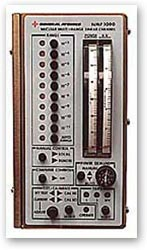
\includegraphics[height=0.4\textheight]{figa/nm1000}
	\mycaption[NM1000]{NM1000.}
	\label{fig:nm1000}
\end{figure}


\section{NP/NPP1000}

The NP1000 and NPP1000 are similar instruments. They are analog ionization chambers, with a range of 10 kW to 2 GW, so they can follow reactor pulses but are mostly useless at startup. They are connected to two types a SCRAM, high power and loss of high voltage.

\begin{figure}[!t]
	\centering
	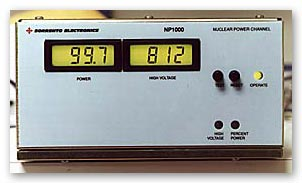
\includegraphics[height=0.4\textheight]{figa/np1000}
	\mycaption[NP/NPP1000]{NP/NPP1000.}
	\label{fig:np1000}
\end{figure}


\
